\begin{frame}
\section{}
Consider the following code snippet for convolution

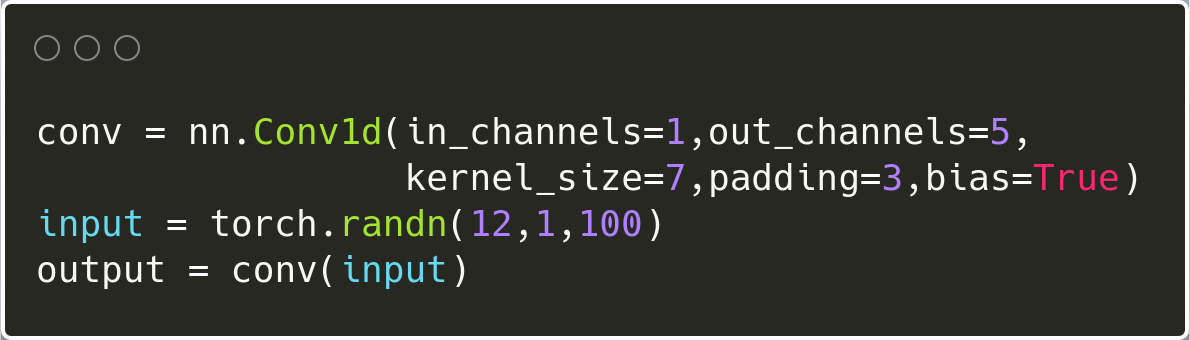
\includegraphics[width=0.7\textwidth]{images/quiz_4_4_4_1.png}

What is the number of trainable parameters in conv?

% FIB

\end{frame}


\begin{frame}
\section{}
Consider the following code snippet for convolution

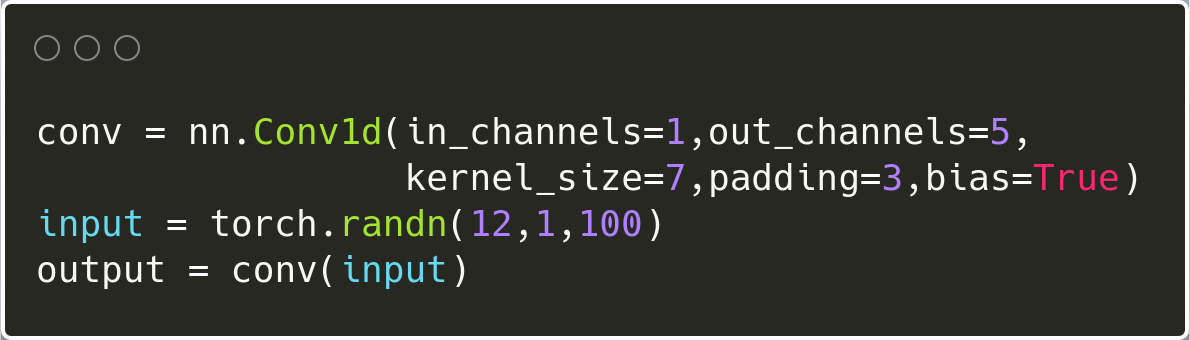
\includegraphics[width=0.7\textwidth]{images/quiz_4_4_4_2.png}

What is the number of trainable parameters in conv?

% FIB

\end{frame}


\begin{frame}
\section{}
Consider the following code snippet for convolution

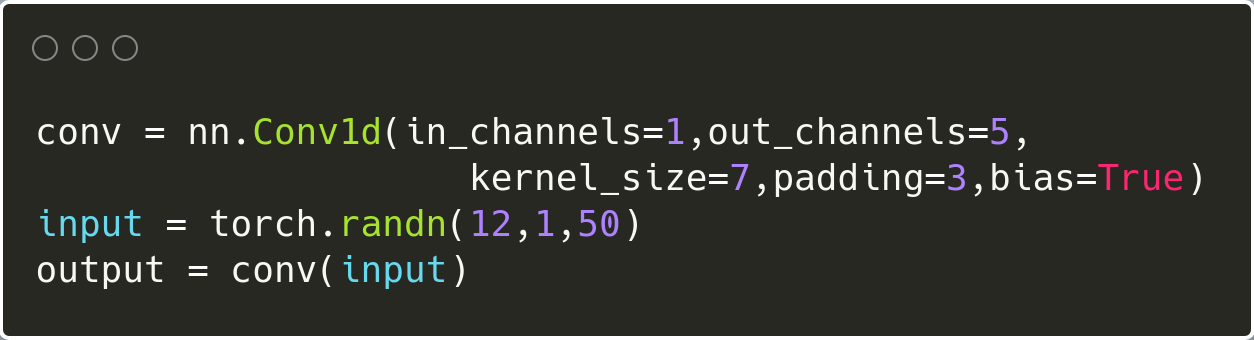
\includegraphics[width=0.7\textwidth]{images/quiz_4_4_4_3.png}

What is the number of trainable parameters in conv?

% FIB

\end{frame}


\begin{frame}
\section{}
Consider the following code snippet for convolution
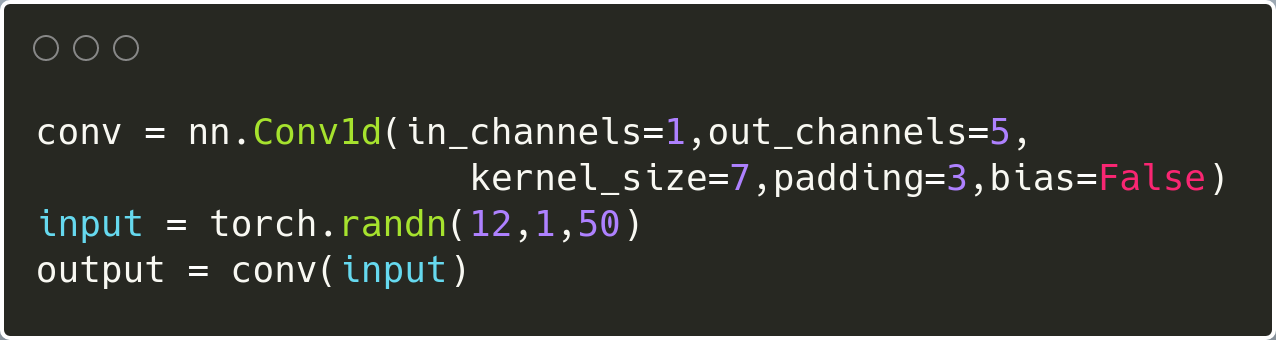
\includegraphics[width=0.7\textwidth]{images/quiz_4_4_4_4.png}


    What is the number of trainable parameters in conv?


% FIB

\end{frame}


\begin{frame}
\section{}
Consider the following code snippet for convolution
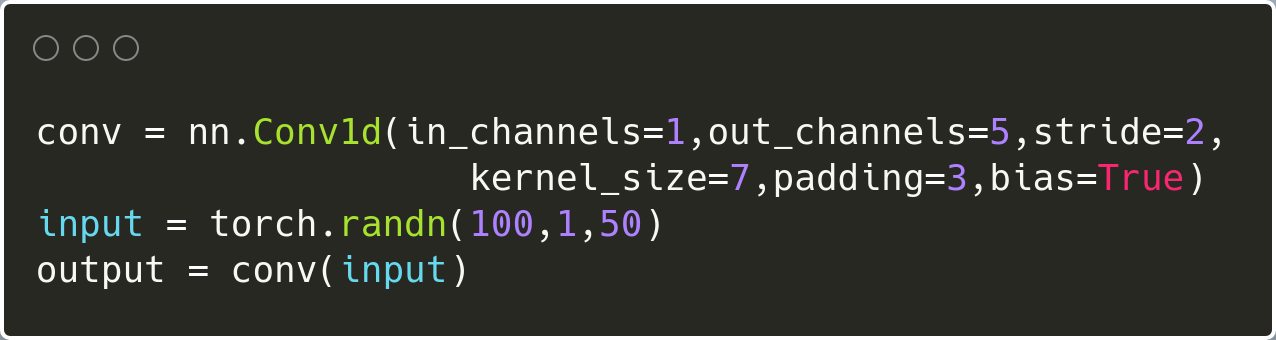
\includegraphics[width=0.7\textwidth]{images/quiz_4_4_4_5.png}

What is the number of trainable parameters in conv?


% FIB

\end{frame}

\begin{frame}
\section{}
Consider the following code snippet for convolution
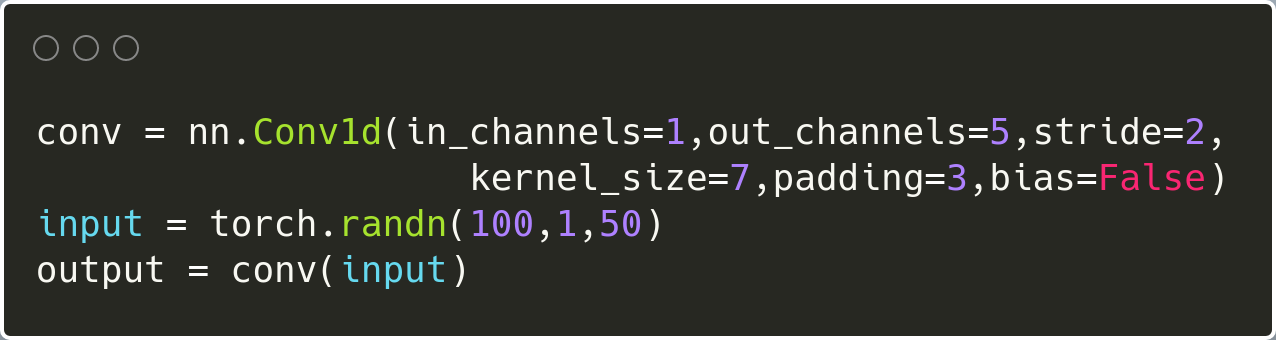
\includegraphics[width=0.7\textwidth]{images/quiz_4_4_4_6.png}

What is the number of trainable parameters in conv?


% FIB

\end{frame}
